\section{Hardware/Software Codesign}
\subsection{Ziele}
	\begin{itemize}
		\item Entwurf (Design) soll so lange wie sinnvoll (nicht so lange wie möglich) lösungsneutral erfolgen
		\item Systemdesign fördern, statt separate Designs für Mechanik, Elektronik, Firmware, Software, etc., die sich unter Umständen auch widersprechen können
		\item Die Systemspezifikation erfolgt idealerweise mit Hilfe einer eindeutigen Spezifikationssprache, nicht in Prosa
		\item Die Spezifikation kann simuliert (ausgeführt) werden
		\item Implementationen können einfach geändert werden, z.B. von HW zu SW oder umgekehrt.
	\end{itemize}

\subsection{Anforderungen für praktische Anwendung}
	\begin{itemize}
		\item Methoden und Tools sollten beim Systemdesign nicht zu fachlastig sein, d.h. die Methoden sollten für Elektronik-, Firmware- und wenn möglich auch Mechanikentwickler anwendbar sein
		\item Falls möglich gute Toolunterstützung und automatische Synthese
	\end{itemize}

\subsection{Spezifikationssprachen}
	\begin{itemize}
		\item Formale Sprachen sind eindeutig
		\item Beispiele für Spezifikationssprachen: SystemC, SysML, SpecC, SystemVerilog, Esterel, Matlab/Simulink, Statecharts
		\item Die Spezifikation kann kompiliert und ausgeführt werden
		\item Simulationen des Systems auf einem leistungsstarken System (z.B. PC) werden meistens unterstützt
		\item Die ausführbare Spezifikation dient als Golden Reference für die künftigen Entwicklungsschritte
	\end{itemize}

\subsection{Virtuelle Prototypen}
	\begin{itemize}
		\item Die Simulation des Systems kann unterschiedlich stark detailliert werden
		\item Die simulierten Systeme sind Virtuelle Prototypen (Mit SystemC/Matlab als Basis sehr gut erreichbar)
		\item Während der Entwicklung können einzelne (virtuelle) Teile des Prototypen laufend durch physische Teile ersetzt werden
	\end{itemize}
\pagebreak\newpage

\subsection{X-in-the-loop}
	\begin{multicols}{2}
		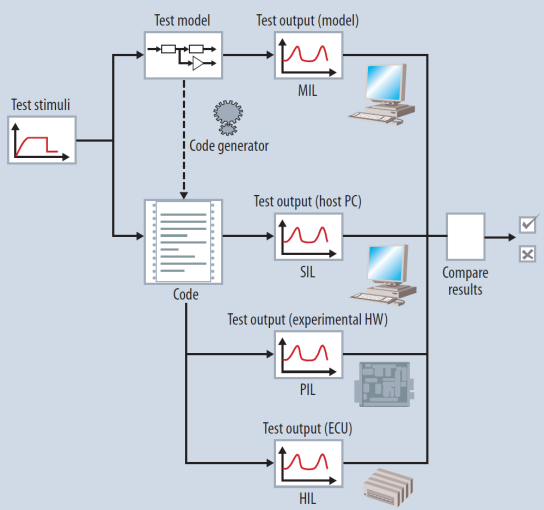
\includegraphics[height=8cm]{images/HWSWCodesign/X-in-the-loop}
		\columnbreak
		\begin{itemize}
			\item Bei einem vollständig als Modell vorliegenden virtuellen Prototyp spricht man auch von Model-in-the-Loop (MIL)
			\item Je mehr der Prototyp durch konkretere Implementationen ersetzt wird, spricht man von
			\begin{itemize}
				\item Software-in-the loop (SIL)
				\item Processor-in-the loop (PIL)
				\item Hardware-in-the loop (HIL)
			\end{itemize}
		\end{itemize}
	\end{multicols}

	\subsection{Entwicklungsplattformen}
	Es eignen sich häufig FPGA-basierte Systeme
	\begin{itemize}
		\item Hardware mit VHDL
		\item Software/Firmware in C/C++
		\begin{itemize}
			\item auf integriertem $\mu$C (Hard core)
			\item auf Softcore innerhalb FPGA
		\end{itemize}
	\end{itemize}
